\documentclass{jarticle}

\usepackage{listings,jlisting} %日本語のコメントアウトをする場合jlistingが必要
%ここからソースコードの表示に関する設定
\lstset{
  basicstyle={\ttfamily},
  identifierstyle={\small},
  commentstyle={\smallitshape},
  keywordstyle={\small\bfseries},
  ndkeywordstyle={\small},
  stringstyle={\small\ttfamily},
  frame={tb},
  breaklines=true,
  columns=[l]{fullflexible},
  numbers=left,
  xrightmargin=0zw,
  xleftmargin=3zw,
  numberstyle={\scriptsize},
  stepnumber=1,
  numbersep=1zw,
  lineskip=-0.5ex
}
%ここまでソースコードの表示に関する設定
\usepackage{comment}
\usepackage[top=30truemm,bottom=30truemm,left=25truemm,right=25truemm]{geometry}
\usepackage[dvipdfmx]{graphicx}
\usepackage{here}

\title{個人進捗報告書}
\author{氏名 織田武瑠}
\date{日付 2019年11月16日提出}

\begin{document}
\maketitle  %文書名・著者名・日付の出力

\section{開発期間2019年11月11日〜11月17日の進捗状況}
\subsection{今回の開発期間の課題と進展事項}
今回の開発期間では,
\begin{itemize}
  \item 遅延が発生しないネットワーク通信プログラムの開発
  \item カメラ実装プログラムとの統合
\end{itemize}
を行った.以下にその詳細を示す.

\subsection{遅延が発生しないネットワーク通信プログラムの開発}
従来のネットワーク通信プログラムでは,プレイヤーの座標が変化する毎にサーバーにクライアントの座標データを送り,その座標データを全クライアントに送っていたため,複数人で実行すると,他のプレイヤーの座標が遅れて表示される現象が発生していた.そこで,クライアントからサーバーには,カーソル操作が変化した時(右カーソルから左カーソルに変化した等)のみ,カーソルの方向情報を送り,サーバーはその情報を全クライアントに送り,各クライアント側で全プレイヤーの座標を計算するというやり方に変更した.これにより,クライアントからの送信回数を大幅に減らせることができたので,遅延も解消できた.

\subsection{カメラ実装プログラムとの統合} 
ネットワーク通信のプログラムとカメラ実装のプログラムを統合した.図\ref{fig:repo1}にカメラ(赤色の三角形)とプレイヤーの様子を示している.プレイヤーがカメラの視野範囲に入ると,3人のプレイヤーの画面から消えるように改良している.

\begin{figure}[H]
\begin{center}
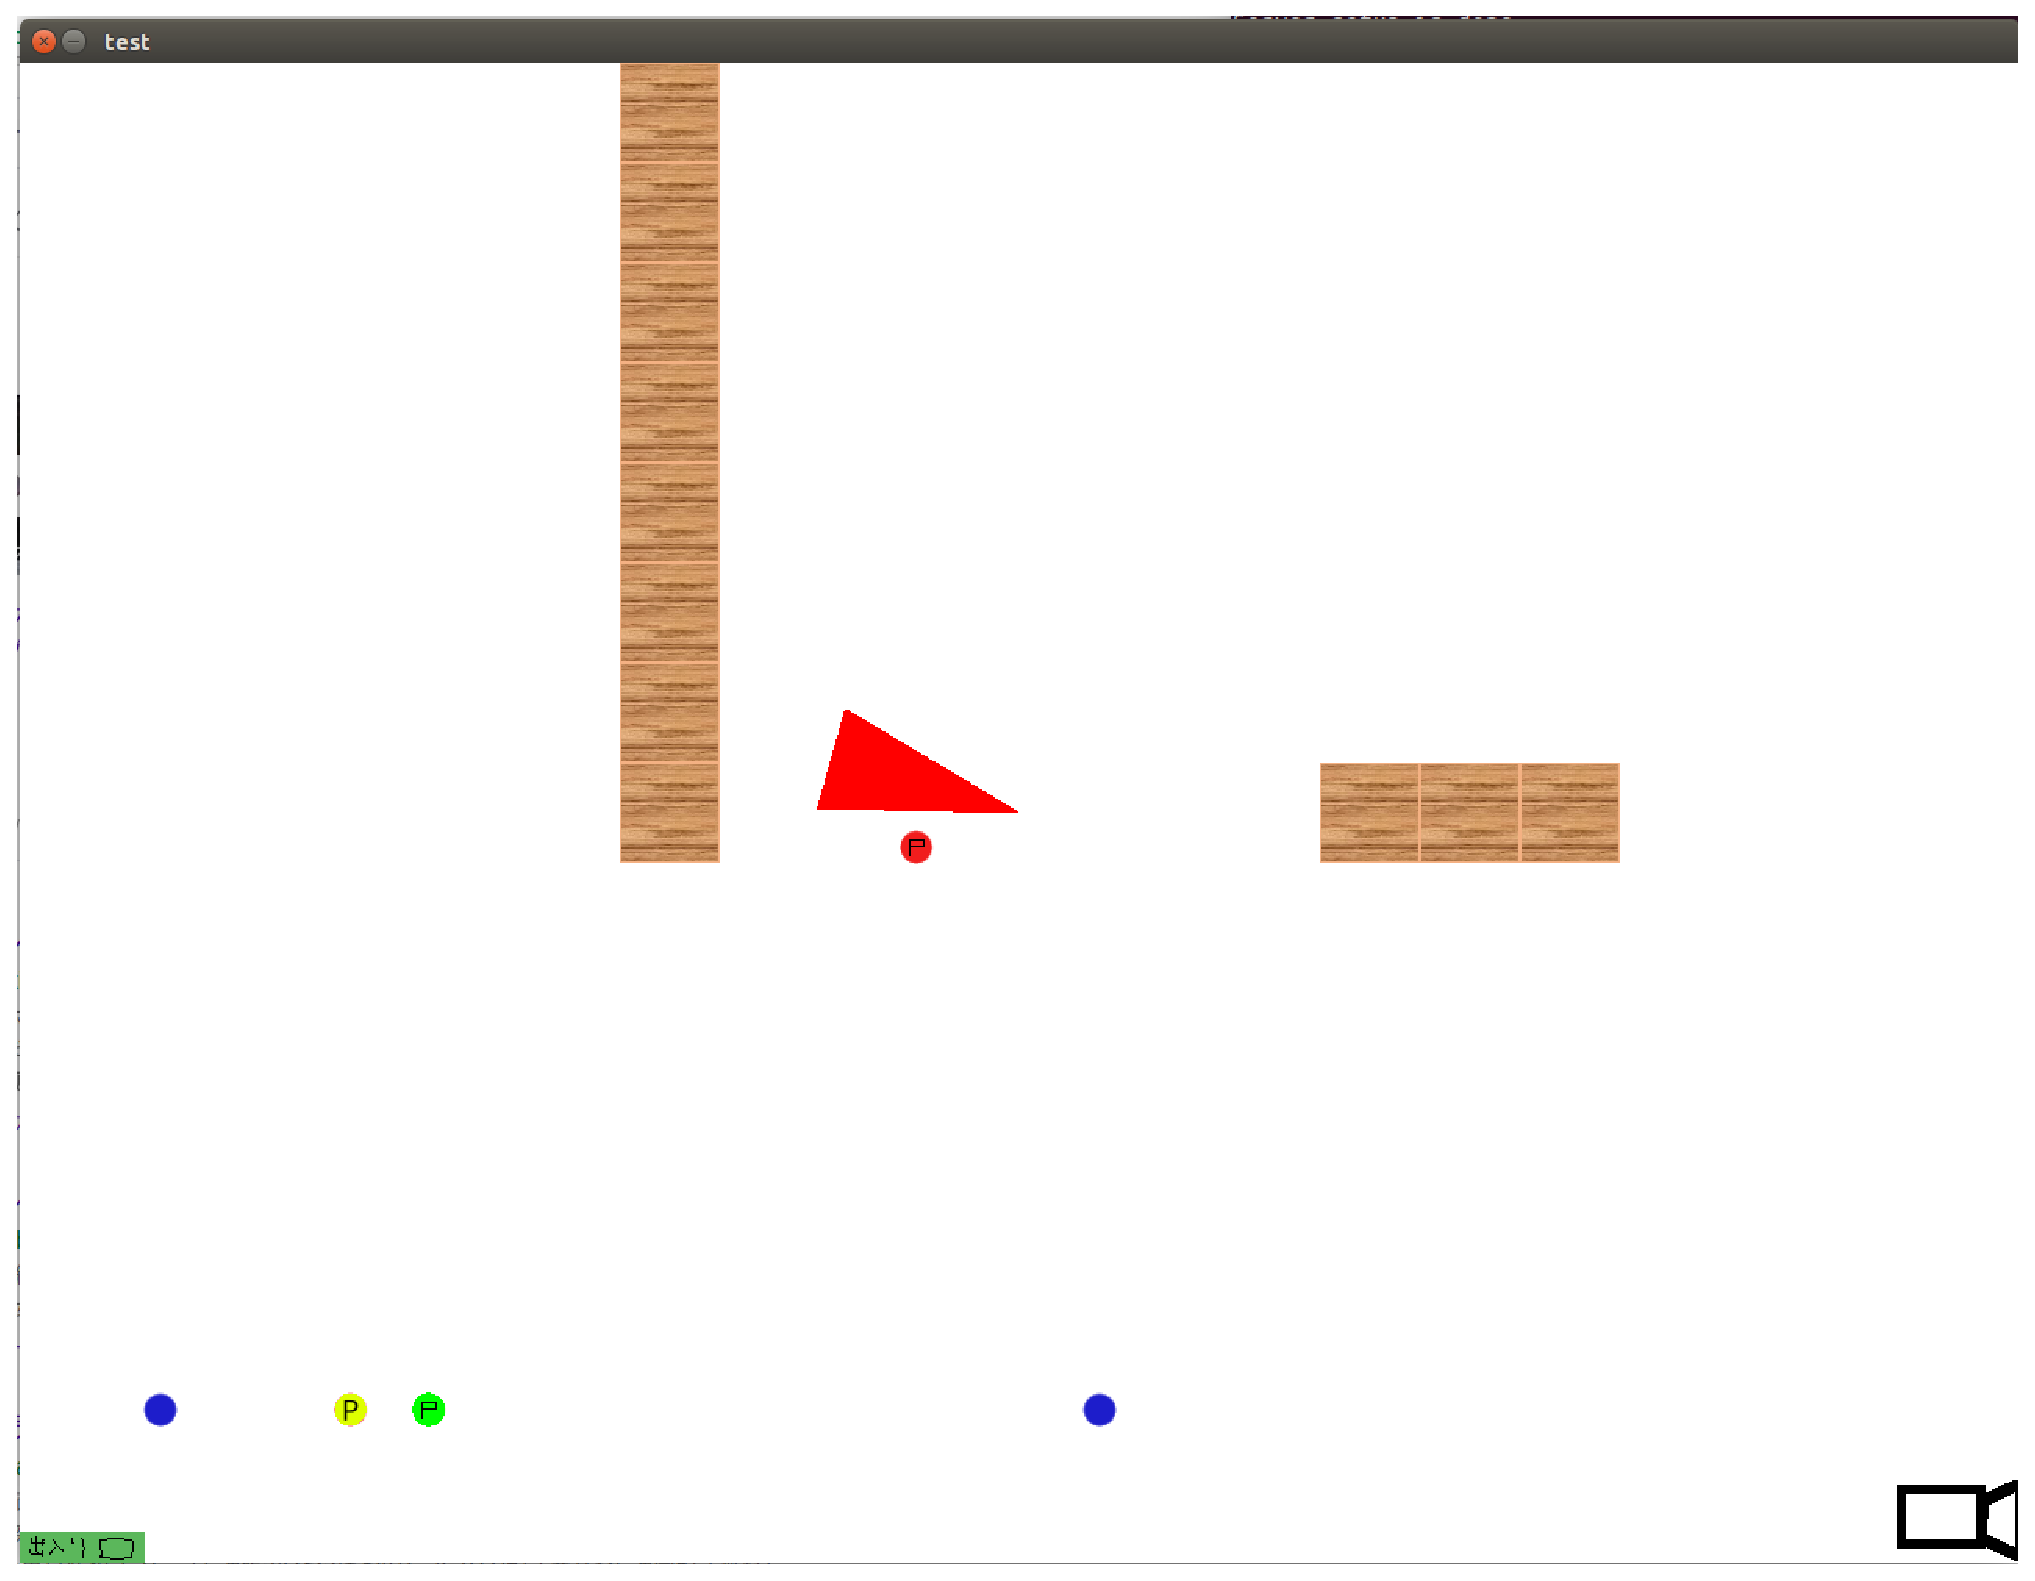
\includegraphics[width=8cm]{pic1.eps}
\caption{カメラとプレイヤーの様子}
\label{fig:repo1}
\end{center}
\end{figure}

\section{開発期間2019年11月18日〜24日の予定}
\begin{itemize}
  \item 複数のカメラの配置を実装したプログラムとの統合
  \item NPCを実装したプログラムとの統合とネットワーク通信化
\end{itemize}

\hspace{3mm}複数のカメラの配置が実装されたので,そのプログラムとネットワーク通信を統合し,よりゲーム性のあるプログラムに進歩させる予定である.
\\\hspace{3mm}現在の問題点として,各プレイヤーがプログラムを実行したタイミングでNPCが動き出しているため,プレイヤーの実行タイミングによって,各プレイヤーの画面で少し,NPCの位置が異なっている,改善策として,3人が実行したのを確認して,NPCの移動が開始されるように変更する予定である.
\end{document}


